
\section{Machine Learning Workloads} \label{sec-ml-workloads}
We define a machine learning workload as a series of exploratory data analysis steps followed by one or multiple model building steps.
Typically users analyze the data by first performing an exploratory analysis.
Then, based on these analyses, they apply the right set of transformations to the data to train one or multiple models on the transformed training data.
Therefore, machine learning workloads typically consist of both interactive (exploratory analysis) and long-running processes (hyperparameter tuning and model training).
Using the experiment database, we can speed up the execution of the machine learning workloads.
By analyzing the experiment database, we can extract the common transformations on data and materialize them.
Thus, during the interactive exploratory analysis, we first analyze the workload to look for reuse opportunities and return the materialized data when possible.
Moreover, using the experiment database, we provide the users with already trained models or promising hyperparameters which decreases the execution time of the hyperparameter search and model training.

We analyzed several scripts from the Titanic: Machine Learning from Disaster competition in Kaggle\footnote{https://www.kaggle.com/c/titanic}.
The Kaggle platform allows users to submit their solutions as scripts (called notebooks or kernels) to the Kaggle platform.
These notebooks are available publicly for other users to view and fork in their own workspace.
Figure \ref{fig-titanic-script-hierarchy} shows some of the popular notebooks and how other users wrote their notebooks based on the existing ones.
The numbers show how many times each script is forked.
The top most-voted notebooks for the Titanic competition have been forked a total of 44,434 times.
This demonstrates that many of the workloads share similar sets of data transformations and model training.
Materializing frequent transformations and models can greatly increase the efficiency and many repeated operations can be avoided.

\begin{figure}
\centering
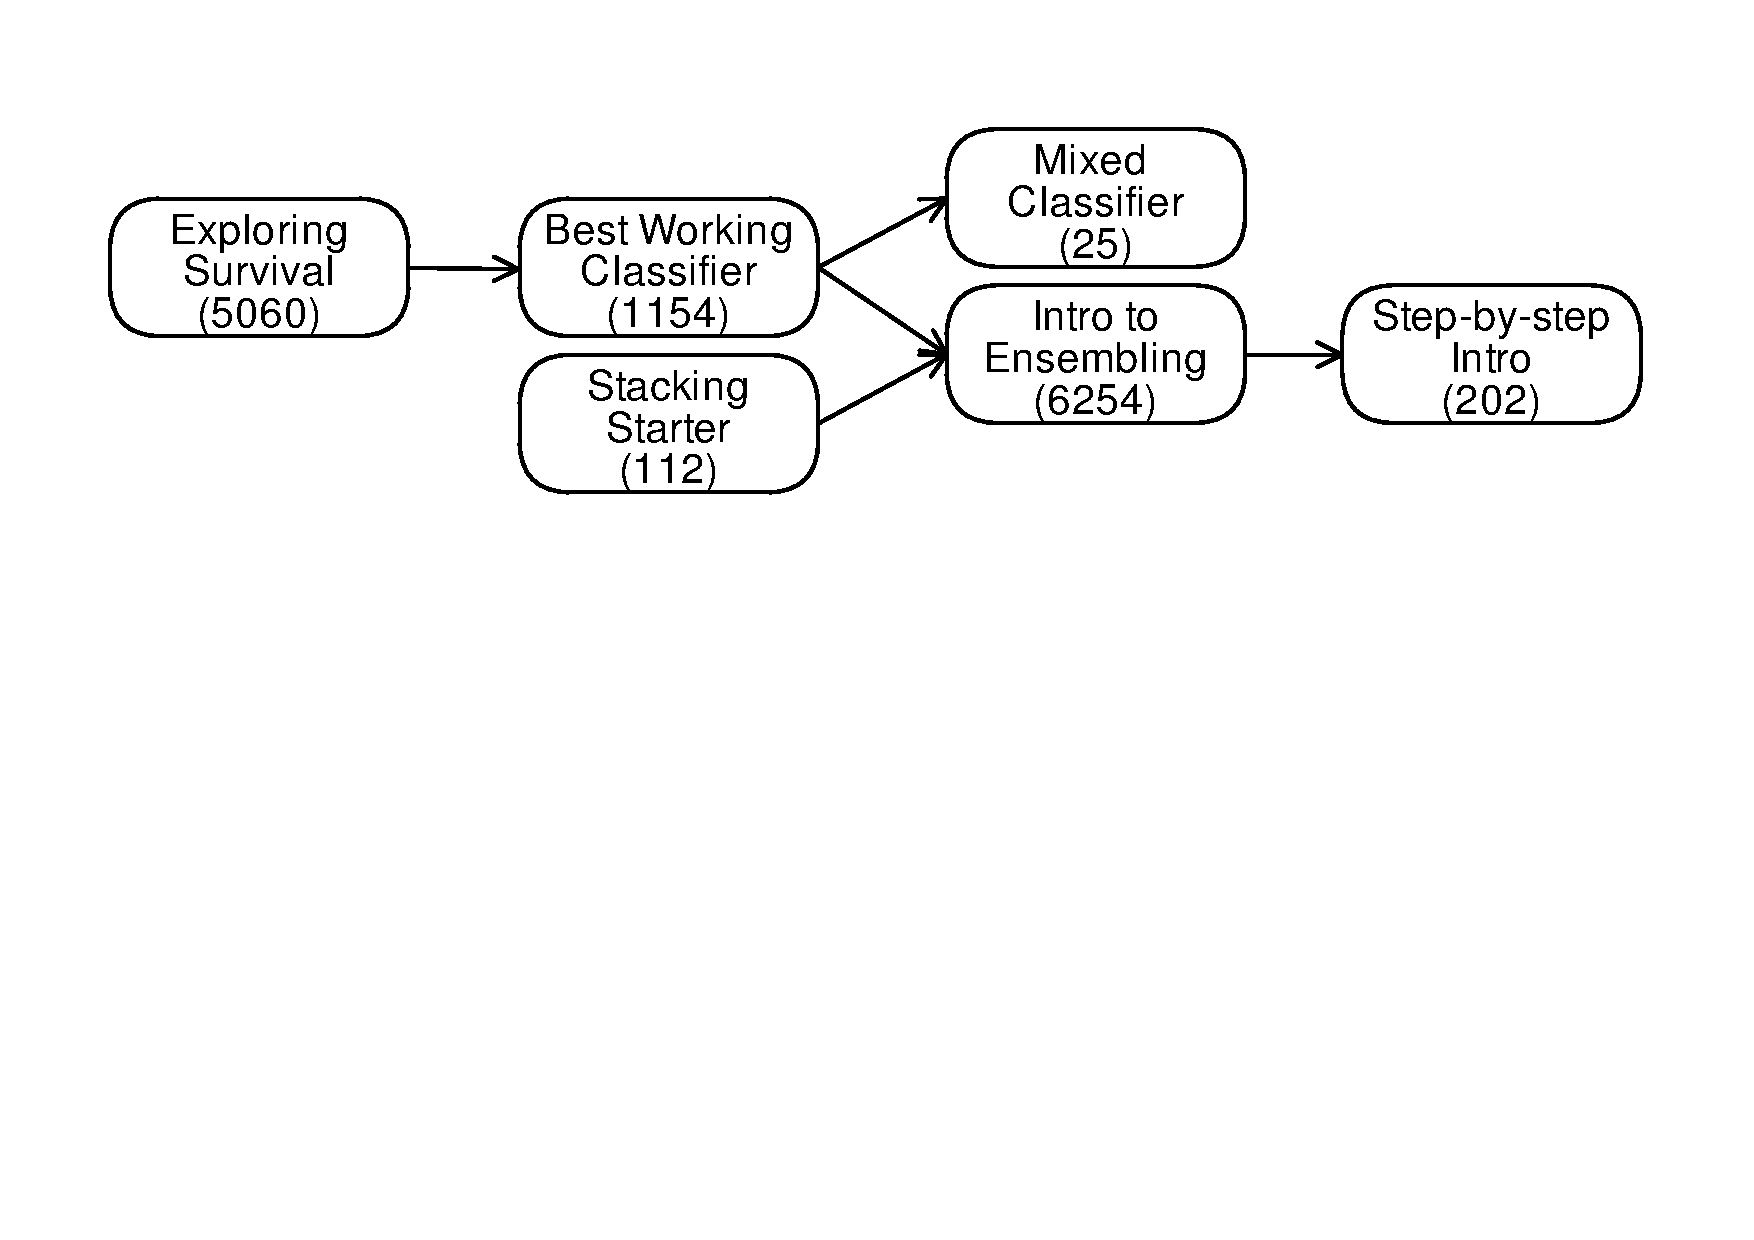
\includegraphics[width=\columnwidth]{../images/kaggle-titanic-scripts-graph}
\caption{The fork hierarchy of some of the popular notebooks in Kaggle's Titanic competition and how many times each notebook is forked}
\label{fig-titanic-script-hierarchy}
\end{figure}

In order to apply the materialization optimization, we first define the characteristics of the machine learning workloads.
Then, we specify how to detect reuse opportunities from the experiment database.

\subsection{Machine Learning Workload Characteristics}
We assume the main units of work are dataframe like objects that contain one or many columns, where all the data items in one column are of one data type.
We divide the operations in the ML workloads into 2 categories.

\begin{table}
\centering
\begin{tabular}{ll}
\hline
	   Feature Extraction & Feature Selection\\ \hline
        feature hasher & variance threshold  \\
        one hot encoding & select k best \\
        count vectorizer& select percentile \\ 
        tfidf transformer & recursive feature elimination \\
        hashing vectorizer & select from model \\
        extract\_patch\_2d &  \\
        \hline
\end{tabular}
\caption{List of feature extraction and feature selection operations}\label{feature-engineering-operations}
\end{table}

\textbf{1. Feature engineering:}
\begin{itemize}
\item feature selection operations
\item feature extraction operations
\item user-define feature engineering operations
\end{itemize}

Table \ref{feature-engineering-operations} shows the list common feature extraction and feature selection operations.

\textbf{2. Model building: }
\begin{itemize}
\item model training operation that applies a training algorithm to a dataset
\item common aggregation operations (such as mean, max, min, and percentile)
\item user-define aggregation operations 
\end{itemize}
Each model building operation results in objects that can either be used in other feature engineering operations (applying PCA to data or categorizing a column based on values in percentile aggregate) or can be a complete machine learning model that can be used to make predictions on unseen data.
\todo[inline]{How can we capture these in the graph? maybe special edges that connect these nodes to a data node? }

%%% Continue from here
\subsection{Graph Construction}
Typically the graph is initially constructed from the experiment database that contains all the historical feature engineering and model building operations.
When new workloads are executed, the graph is extended to capture the new feature engineering and model building operations.
The process of constructing the graph is as follows.
First, a node (root) which represents the (training) dataset is created.
Since operations are performed on columns of the dataset, an edge is drawn for every column of the data from the root to new vertices representing every column of the data.
Every operation represents an edge.
Edge connects a starting node (one or more columns of the data) to another node (the resulting columns).
If the feature engineering operations is known, the edge also stores information about the feature engineering operation applied.
the resulting node of the operation contains the columns of data resulted from applying the operation.

Model building operations also operate on one or more columns of the data.
Similar to the feature engineering operation, an edge represent the operation.
If the operation is not a user-defined aggregation operation, the edge carries information about the operation (such as training algorithm and hyper-parameters).
The resulting node represents a machine learning model (for model training operations) or data structures keeping the aggregated values (for aggregation operations).

Figure \ref{fig-experiment-graph} shows an example graph constructed from the code in Listing \ref{listing-experiment-graph}.

\begin{lstlisting}[language=Python, caption=Example script,captionpos=b,label = {listing-experiment-graph}]
import numpy as np
import pandas as pd

from sklearn import svm
from sklearn.feature_selection import SelectKBest
from sklearn.feature_extraction.text import CountVectorizer

train = pd.read_csv('../input/train.csv')
vectorizer = CountVectorizer()
count_vectorized = vectorizer.fit_transform(train['ad_description'])
selector =  SelectKBest(k=2)
top_features = selector.fit_transform(train[['t','u_id','price']], train['y'])
X = pd.concat([count_vectorized,top_features], axis = 1)
model = svm.SVC()
model.fit(X, train['y'])
\end{lstlisting}

\begin{figure}
\centering
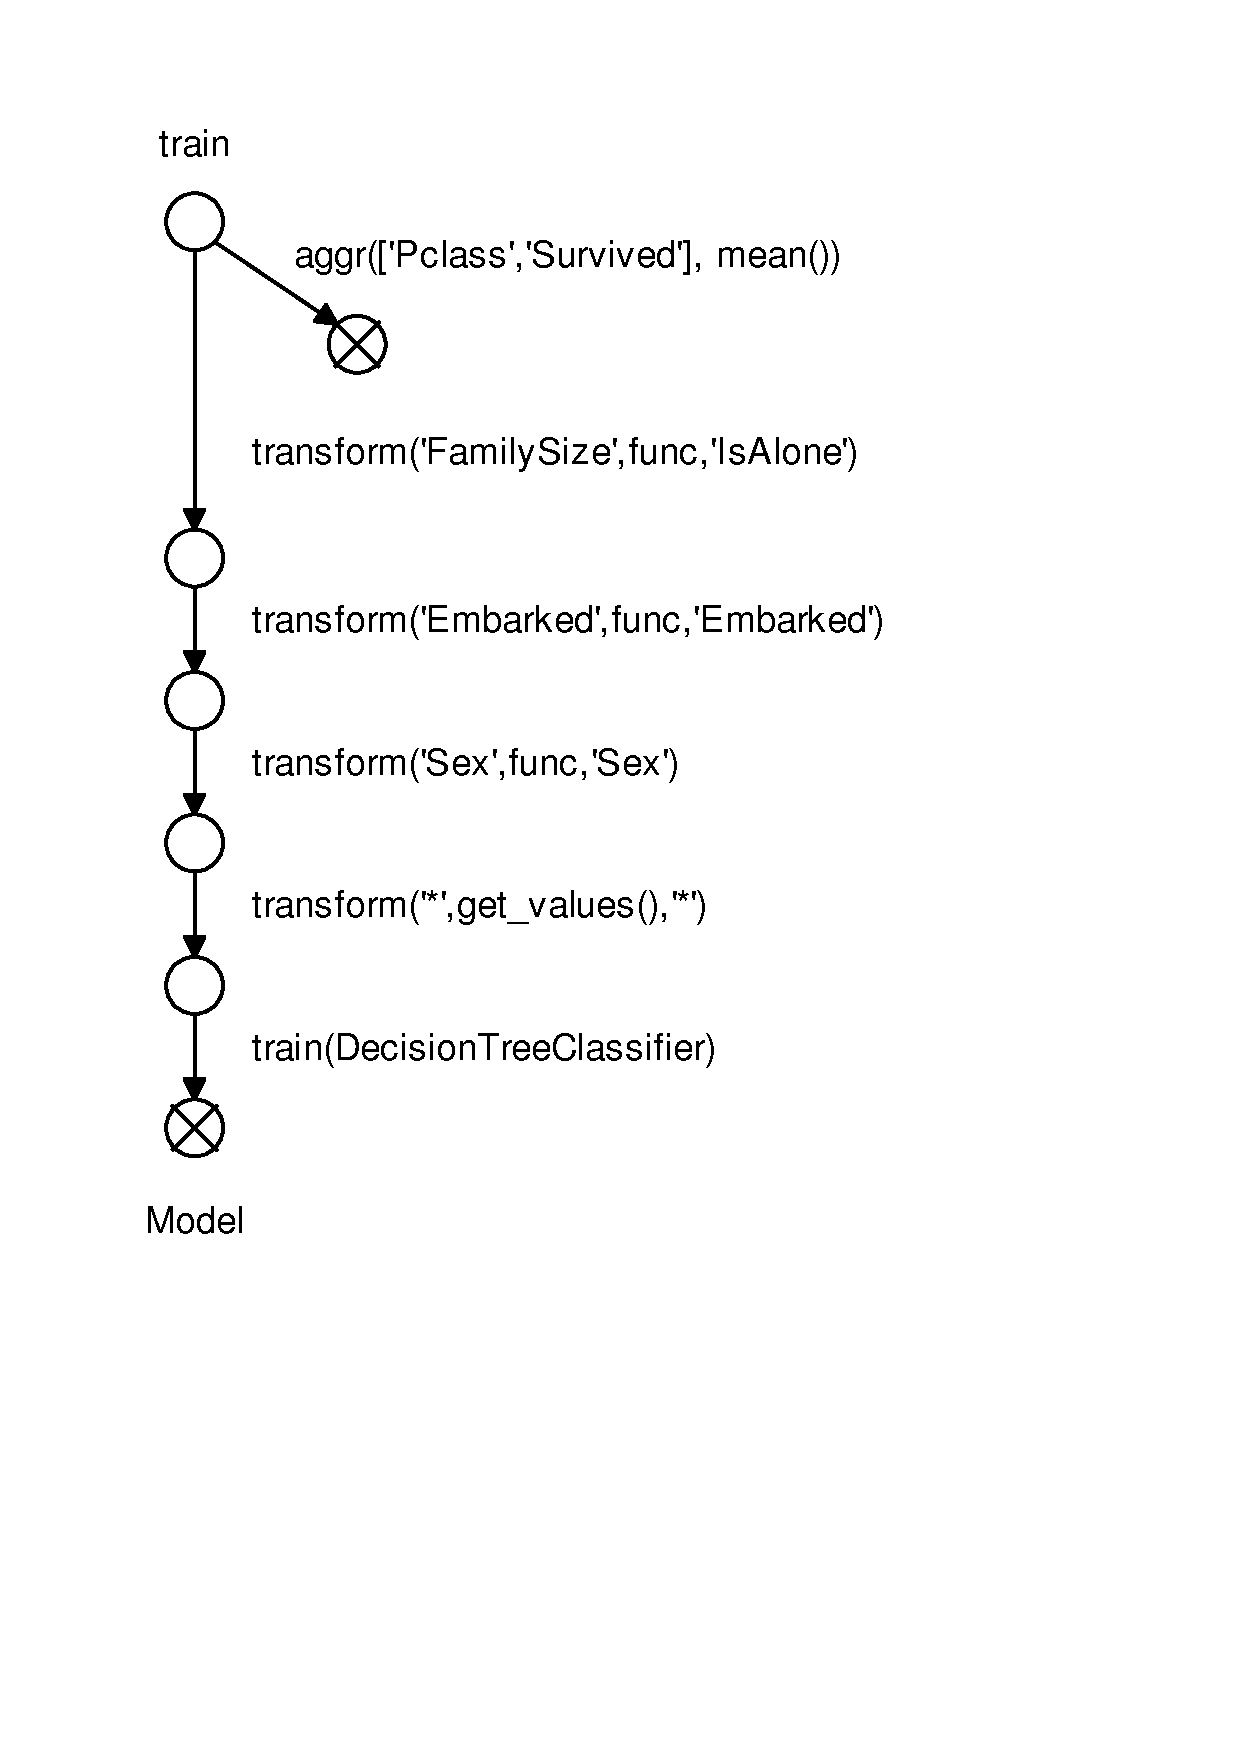
\includegraphics[width=\columnwidth]{../images/experiment-graph}
\caption{Experiment graph constructed from the Listing \ref{listing-experiment-graph}}
\label{fig-experiment-graph}
\end{figure}
